\subsection{Modeling DUR Processing Time}\label{modeling-dur-processing-time}

A model was built to predict DUR durations for the following reasons:

\begin{itemize}
\tightlist
\item
  The analysis
  \href{https://chewyinc.atlassian.net/wiki/x/hYRyRQE}{Would Grouping
  Similar Work Make Pharmacists Faster? What the data says} concludes
  that the previous task has no effect. We would like to know whether
  the result changes after controlling for factors other than MC3,
  cohort, or part number. We also want to determine whether another
  definition of similarity is more appropriate and quantify the
  uncertainty in the estimate.
\end{itemize}

Consider two task sequences from the same user:

Both sequences have MC3 \texttt{Parasiticide} and approval channel
\texttt{PH}. All start times have UTC offset \texttt{+0000} and
\texttt{.000} milliseconds; blank updated fields mean no fields were
updated.

Sequence A: pet \texttt{Dog}, initiation channel \texttt{AUTOSHIP}.

{\def\LTcaptype{none} % do not increment counter
\begin{longtable}[]{@{}rrrll@{}}
\toprule\noalign{}
Order & Part number & Duration (s) & Start time (UTC) & Updated
fields \\
\midrule\noalign{}
\endhead
\bottomrule\noalign{}
\endlastfoot
1 & 146066 & 40 & 2026-04-30 06:42:54 & \\
2 & 152702 & 27 & 2026-04-30 06:43:36 & directions \\
3 & 146391 & 40 & 2026-04-30 06:44:06 & \\
4 & 151583 & 7 & 2026-04-30 06:44:48 & \\
5 & 146138 & 7 & 2026-04-30 06:44:56 & \\
6 & 146142 & 43 & 2026-04-30 06:45:05 & directions \\
7 & 146142 & 35 & 2026-04-30 06:45:49 & directions \\
8 & 146064 & 39 & 2026-04-30 06:46:26 & directions \\
9 & 146167 & 12 & 2026-04-30 06:47:07 & \\
10 & 146322 & 9 & 2026-04-30 06:47:21 & directions \\
11 & 146167 & 97 & 2026-04-30 06:47:32 & directions \\
12 & 146050 & 6 & 2026-04-30 06:49:11 & \\
13 & 146387 & 54 & 2026-04-30 06:49:19 & \\
\end{longtable}
}

Sequence B: pet \texttt{Cat}, initiation channel \texttt{OMS}.

{\def\LTcaptype{none} % do not increment counter
\begin{longtable}[]{@{}rrrll@{}}
\toprule\noalign{}
Order & Part number & Duration (s) & Start time (UTC) & Updated
fields \\
\midrule\noalign{}
\endhead
\bottomrule\noalign{}
\endlastfoot
1 & 158995 & 11 & 2026-07-15 02:17:23 & \\
2 & 158995 & 35 & 2026-07-15 02:17:36 & \\
3 & 158995 & 3 & 2026-07-15 02:18:13 & \\
4 & 158995 & 13 & 2026-07-15 02:18:17 & \\
5 & 158995 & 13 & 2026-07-15 02:18:31 & \\
6 & 158995 & 6 & 2026-07-15 02:18:46 & \\
7 & 158995 & 16 & 2026-07-15 02:18:53 & \\
8 & 158995 & 13 & 2026-07-15 02:19:11 & \\
9 & 158995 & 6 & 2026-07-15 02:19:25 & \\
10 & 158995 & 50 & 2026-07-15 02:19:32 & \\
11 & 158998 & 11 & 2026-07-15 02:20:23 & \\
12 & 158998 & 29 & 2026-07-15 02:20:36 & \\
\end{longtable}
}

The model predicts a statistically significant effect when the preceding
task is "similar" for a user. However, substantial unexplained variation
remains.

The predicted effect at several baseline DUR durations is:

\begingroup\setlength{\tabcolsep}{5pt}

{\def\LTcaptype{none} % do not increment counter
\begin{longtable}[]{@{}rrrrrr@{}}
\toprule\noalign{}
Without same preceding & With same preceding & -1 residual SD & +1
residual SD & Difference & Change (\%) \\
\midrule\noalign{}
\endhead
\bottomrule\noalign{}
\endlastfoot
15.00 s & 14.16 s & 6.84 s & 30.70 s & -0.84 s & -5.58\% \\
50.00 s & 46.93 s & 21.09 s & 110.44 s & -3.07 s & -6.14\% \\
150.00 s & 139.96 s & 58.53 s & 357.84 s & -10.04 s & -6.69\% \\
\end{longtable}
}

\endgroup

The model predicts that users and products differ in processing speed,
while day of the week has no statistically significant effect.

The model also predicts longer DUR times when prescription data are
altered.

How reliable are our estimates for hypothetical sequencing scenarios?

\subsubsection{EDA on Factors Affecting
DUR}\label{eda-on-factors-affecting-dur}

See \hyperref[factors-affecting-successful-durs]{Factors Affecting DUR}
in the Appendix.

We assume that the following groups of factors affect DUR duration:

\begin{enumerate}
\def\labelenumi{\arabic{enumi}.}
\tightlist
\item
  The user

  \begin{itemize}
  \tightlist
  \item
    Are some users inherently slower? Are they consistently slower or
    faster across cohorts?
  \end{itemize}
\item
  The prescription

  \begin{itemize}
  \tightlist
  \item
    Medication
  \item
    Content (typos, missing information)
  \item
    Pet

    \begin{itemize}
    \tightlist
    \item
      Pet health history
    \end{itemize}
  \end{itemize}
\item
  Business process
\item
  Outside disturbances, such as inbound calls
\item
  The user\textquotesingle s task history

  \begin{itemize}
  \tightlist
  \item
    Did they perform similar tasks previously?
  \end{itemize}
\item
  Environment
\item
  Software platform
\end{enumerate}

A more detailed breakdown can be found
\href{../../charts/DUR_detailed.png}{here}.

For details, see \hyperref[model-details]{Model Details} in the
Appendix.


\paragraph{Model Details}\label{model-details}

\subparagraph{Final MC3/COH/PETTYPE mixed-effects
model}\label{final-mc3cohpettype-mixed-effects-model}

The model is built to understand the factors affecting approved DUR task
durations. It uses MC3, cohort, and pet type to define groups of similar
DUR tasks.

The model controls for weekday, approval channel, prescription source,
parent part number, user (for example, pharmacist or pharmacy
technician), and changes to prescription data, such as updated
directions.

There are two treatments based on whether the current task is adjacent
to another task in the same MC3, cohort, and pet type equivalence class
for a given user. Adjacent tasks must be no more than one hour apart.
Failed DURs and DUR tasks that overlap in time with other DUR tasks are
excluded; these cases occur for certain orders. If a preceding task
belongs to the same equivalence class, the \texttt{SAME\_PRECEDING}
treatment is true. If the following task belongs to the same equivalence
class, the \texttt{SAME\_FOLLOWING} treatment is true.
\texttt{SAME\_FOLLOWING} is expected to have a coefficient near zero. It
exists to check whether the model captures confounding factors
adequately.

The model estimates each user\textquotesingle s deviation from mean
performance. It does the same for each parent part number and each
calendar date.

The model predicts that, for a given user, a task preceded by a task in
the same cell has a shorter DUR duration. After controlling for MC3,
cohort, pet type, and parent part number, the model finds no
statistically significant association with \texttt{SAME\_FOLLOWING}.

The weekday fixed effects are not statistically significant, whereas
some approval-channel and prescription-source effects are.
Customer-originated prescriptions take longer.

\subparagraph{Purpose and analysis
sample}\label{purpose-and-analysis-sample}

This is the final model. It estimates how same-cell sequence position
relates to DUR duration while controlling for correction status,
weekday, approval channel, prescription source, and MC3/COH/PETTYPE
cell. It includes crossed random intercepts for user, process date, and
parent part number.

The source is
\texttt{EDLDB\_DEV.PET\_HEALTH\_ANALYTICS\_SANDBOX.MY\_RXP\_VALID\_DUR\_TASKS}.
Eligible rows have non-null user, task, process-start time,
\texttt{MC3\_COH\_PETTYPE\_SEQN}, and
\texttt{MC3\_COH\_PETTYPE\_BATCH\_LEN}; sequence and batch length are at
least one, and sequence does not exceed batch length. Duration is
\texttt{IMPUTED\_DWELL\_IN\_PROGRESS\_TO\_CLOSED\_SECONDS}.

Let \(Y_i\) be the positive imputed duration in seconds for task \(i\).
One global cutoff is calculated over all otherwise eligible tasks with
Snowflake\textquotesingle s \texttt{APPROX\_PERCENTILE(Y,\ 0.95)}
function call:

\[
q_{0.95}=Q_{0.95}(Y).
\]

The fitted sample keeps tasks satisfying \(0<Y_i<q_{0.95}\); the upper
bound is strict. MC3, COH, PETTYPE, parent part number, approval
channel, and prescription source blanks are represented by
\texttt{\textless{}Missing\textgreater{}}.

\subparagraph{Derived indicators}\label{derived-indicators}

For sequence number \(S_i\), batch length \(L_i\), and correction count
\(N_i\), the three binary fixed effects are

\[
P_i=\mathbf{1}(L_i>1\ \land\ S_i>1),
\qquad
F_i=\mathbf{1}(L_i>1\ \land\ S_i<L_i),
\qquad
C_i=\mathbf{1}(N_i>0).
\]

Thus \(P_i\) is \texttt{SAME\_PRECEDING}, \(F_i\) is
\texttt{SAME\_FOLLOWING}, and \(C_i\) is \texttt{HAS\_CORRECTION}.

\subparagraph{Outcome transformation}\label{outcome-transformation}

The retained durations receive one global Box-Cox transformation:

\[
Z_i=g_\lambda(Y_i)=
\begin{cases}
\dfrac{Y_i^\lambda-1}{\lambda}, & \lambda\ne0,\\
\log(Y_i), & \lambda=0.
\end{cases}
\]

The maximum-likelihood transformation estimate is
\(\widehat{\lambda}=-0.08159843\). All coefficients, random effects,
standard deviations, residuals, RMSE, and diagnostics are therefore on
the Box-Cox scale.

\subparagraph{Complete model formula}\label{complete-model-formula}

Index task, fixed-effect cell, user, date, and parent part by
\(i, c, u, d, p\). The model is

\[
\begin{aligned}
Z_i={}&\gamma_{c(i)}+\beta_P P_i+\beta_F F_i+\beta_C C_i\\
&+\sum_{w\ne\mathrm{Sun}}\delta_w\mathbf{1}(W_i=w)\\
&+\sum_{a\ne a_0}\theta_a\mathbf{1}(A_i=a)
+\sum_{s\ne s_0}\phi_s\mathbf{1}(R_i=s)\\
&+b_{u(i)}+h_{d(i)}+r_{p(i)}+\epsilon_i.
\end{aligned}
\]

Here \(\gamma_{c(i)}\) is a fixed effect shared by all tasks in the same
MC3 + COH + PETTYPE cell. The model uses a full set of cell effects and
no separate overall intercept. Sunday is the weekday reference. The
data-dependent categorical references are:

\begin{itemize}
\tightlist
\item
  approval channel \(a_0\): \texttt{PH}
\item
  prescription source \(s_0\): \texttt{PRACTICE\_HUB}
\end{itemize}

Each reference is the most frequent retained level; lexicographic order
breaks a frequency tie. The crossed random terms and level-1 error are
mutually independent and satisfy

\[
b_u\sim N(0,\sigma_u^2),\qquad
h_d\sim N(0,\sigma_d^2),\qquad
r_p\sim N(0,\sigma_p^2),\qquad
\epsilon_i\sim N(0,\sigma_e^2).
\]

The fixed effects and variance components are estimated jointly by REML.
The conditional fitted value and residual are

\[
\widehat{Z}_i=\widehat{\gamma}_{c(i)}+x_i^T\widehat{\beta}
+\widehat{b}_{u(i)}+\widehat{h}_{d(i)}+\widehat{r}_{p(i)},
\qquad e_i=Z_i-\widehat{Z}_i.
\]

\subparagraph{Inference and fit
statistics}\label{inference-and-fit-statistics}

For fixed effect \(k\), the report uses

\[
z_k=\frac{\widehat{\beta}_k}{\mathrm{SE}(\widehat{\beta}_k)},\qquad
p_k=2\Phi(-\lvert z_k\rvert),\qquad
\mathrm{CI}_{95}=\widehat{\beta}_k\pm1.96\,\mathrm{SE}(\widehat{\beta}_k).
\]

The fixed-effect table labels an estimate \texttt{Significant\ =\ Yes}
when its 95\% confidence interval excludes zero; intervals that cross or
touch zero are marked \texttt{No}.

Random-effect SD intervals use an observed-information Wald
approximation on the log-SD scale. The residual-SD interval uses the
chi-square distribution. The reported conditional metrics include all
fixed and random effects:

\[
R_c^2=1-\frac{\sum_i e_i^2}{\sum_i(Z_i-\bar Z)^2},\qquad
RMSE_c=\sqrt{\frac1n\sum_i e_i^2}.
\]

\Needspace{8\baselineskip}

\subparagraph{Sample and fit}\label{sample-and-fit}

{\def\LTcaptype{none} % do not increment counter
\begin{longtable}[]{@{}lr@{}}
\toprule\noalign{}
Quantity & Value \\
\midrule\noalign{}
\endhead
\bottomrule\noalign{}
\endlastfoot
Tasks & 3,433,218 \\
MC3/COH/PETTYPE cells & 265 \\
Users & 340 \\
Dates & 182 \\
Parent part numbers & 885 \\
Approval-channel levels & 9 \\
Prescription-source levels & 11 \\
Global approximate P95 cutoff (seconds) & 156.598673 \\
Box-Cox lambda & -0.08159843 \\
Conditional R-squared & 0.308784 \\
Conditional RMSE (Box-Cox scale) & 0.603674 \\
REML negative log-likelihood & 3142827.127402 \\
Converged & True \\
\end{longtable}
}

\subparagraph{Fixed effects}\label{fixed-effects}

In the term column, \texttt{AC} denotes approval-channel effects
relative to \texttt{PH}; \texttt{PS} denotes prescription-source effects
relative to \texttt{PRACTICE\_HUB}.

\begingroup\setlength{\tabcolsep}{4pt}

{\def\LTcaptype{none} % do not increment counter
\begin{longtable}[]{@{}lrrrrrc@{}}
\toprule\noalign{}
Term & Estimate & SE & z & p-value & 95\% CI & Significant \\
\midrule\noalign{}
\endhead
\bottomrule\noalign{}
\endlastfoot
SAME\_PRECEDING & -0.046157 & 0.000835 & -55.2813 & \textless1e-300 &
{[}-0.047793, -0.044520{]} & Yes \\
SAME\_FOLLOWING & 0.001024 & 0.000835 & 1.2259 & 0.220231 &
{[}-0.000613, 0.002661{]} & No \\
HAS\_CORRECTION & 0.271146 & 0.000788 & 344.0672 & \textless1e-300 &
{[}0.269601, 0.272690{]} & Yes \\
WEEKDAY\_MON & 0.006416 & 0.019649 & 0.3265 & 0.74404 & {[}-0.032096,
0.044927{]} & No \\
WEEKDAY\_TUE & 0.014299 & 0.019646 & 0.7278 & 0.466718 & {[}-0.024206,
0.052803{]} & No \\
WEEKDAY\_WED & 0.010462 & 0.019650 & 0.5324 & 0.59444 & {[}-0.028051,
0.048975{]} & No \\
WEEKDAY\_THU & 0.008138 & 0.019652 & 0.4141 & 0.678785 & {[}-0.030379,
0.046655{]} & No \\
WEEKDAY\_FRI & 0.006015 & 0.019651 & 0.3061 & 0.75952 & {[}-0.032499,
0.044530{]} & No \\
WEEKDAY\_SAT & 0.002131 & 0.019666 & 0.1084 & 0.913702 & {[}-0.036413,
0.040675{]} & No \\
AC: CLINIC\_EMAIL & 0.235910 & 0.045211 & 5.2180 & 1.80853e-07 &
{[}0.147299, 0.324522{]} & Yes \\
AC: CUSTOMER\_MAIL & 0.472534 & 0.013061 & 36.1785 & 1.32431e-286 &
{[}0.446934, 0.498133{]} & Yes \\
AC: DIGITAL & 0.146802 & 0.040724 & 3.6048 & 0.000312369 & {[}0.066985,
0.226619{]} & Yes \\
AC: FAX & 0.208015 & 0.011227 & 18.5276 & 1.23668e-76 & {[}0.186010,
0.230020{]} & Yes \\
AC: PARTNER & -0.034275 & 0.007967 & -4.3018 & 1.69381e-05 &
{[}-0.049891, -0.018659{]} & Yes \\
AC: RHAPSODY & 0.075320 & 0.052573 & 1.4327 & 0.15195 & {[}-0.027721,
0.178362{]} & No \\
AC: VERBAL & -0.017687 & 0.010665 & -1.6585 & 0.097222 & {[}-0.038589,
0.003215{]} & No \\
AC: VET & 0.003570 & 0.105720 & 0.0338 & 0.973059 & {[}-0.203638,
0.210779{]} & No \\
PS: CLINIC\_EMAIL & -0.003227 & 0.011181 & -0.2886 & 0.772878 &
{[}-0.025141, 0.018687{]} & No \\
PS: CS\_FIRST\_CONTACT & -0.086051 & 0.203897 & -0.4220 & 0.673003 &
{[}-0.485682, 0.313580{]} & No \\
PS: CUSTOMER\_MAIL & 0.044423 & 0.012813 & 3.4672 & 0.000525987 &
{[}0.019311, 0.069536{]} & Yes \\
PS: CVC & 0.023167 & 0.052511 & 0.4412 & 0.659085 & {[}-0.079753,
0.126087{]} & No \\
PS: DIGITAL & 0.020414 & 0.040106 & 0.5090 & 0.610753 & {[}-0.058192,
0.099020{]} & No \\
PS: FAX & -0.004739 & 0.011224 & -0.4222 & 0.67286 & {[}-0.026738,
0.017260{]} & No \\
PS: PARTNER\_API & 0.018961 & 0.007944 & 2.3869 & 0.0169906 &
{[}0.003392, 0.034530{]} & Yes \\
PS: RHAPSODY & -0.029700 & 0.062733 & -0.4734 & 0.6359 & {[}-0.152655,
0.093254{]} & No \\
PS: TELEMEDICINE & 0.185396 & 0.052942 & 3.5018 & 0.000462051 &
{[}0.081631, 0.289161{]} & Yes \\
PS: VERBAL & -0.002803 & 0.011736 & -0.2388 & 0.81126 & {[}-0.025805,
0.020200{]} & No \\
\end{longtable}
}

\endgroup

\Needspace{8\baselineskip}

\subparagraph{Variance components}\label{variance-components}

{\def\LTcaptype{none} % do not increment counter
\begin{longtable}[]{@{}lrr@{}}
\toprule\noalign{}
Component & SD & Approximate 95\% CI \\
\midrule\noalign{}
\endhead
\bottomrule\noalign{}
\endlastfoot
User random intercept & 0.422318 & {[}0.390500, 0.456728{]} \\
Date random intercept & 0.070610 & {[}0.063513, 0.078500{]} \\
Parent-part random intercept & 0.114187 & {[}0.107719, 0.121045{]} \\
Residual & 0.603803 & {[}0.603351, 0.604255{]} \\
\end{longtable}
}

\subparagraph{Diagnostics}\label{diagnostics}

\pandocbounded{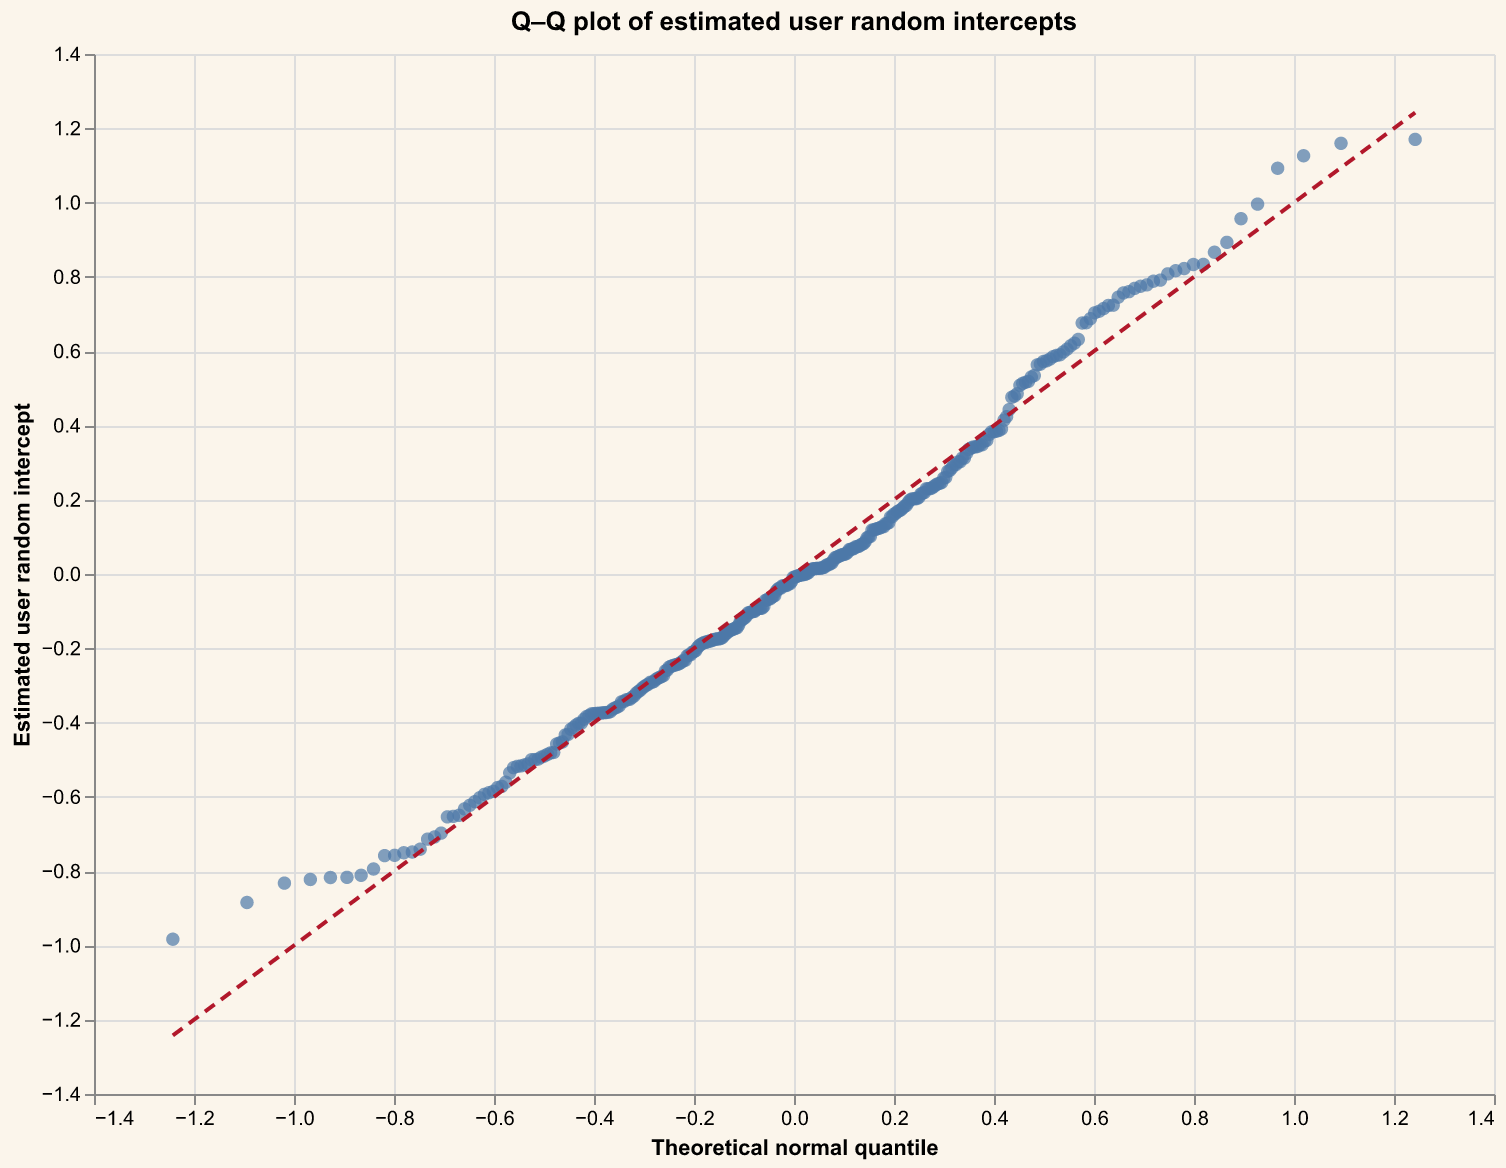
\includegraphics[keepaspectratio,alt={User Q--Q plot}]{outputs/charts/mc3-coh-pettype-final-model/user_random_intercepts_qq.png}}

\pandocbounded{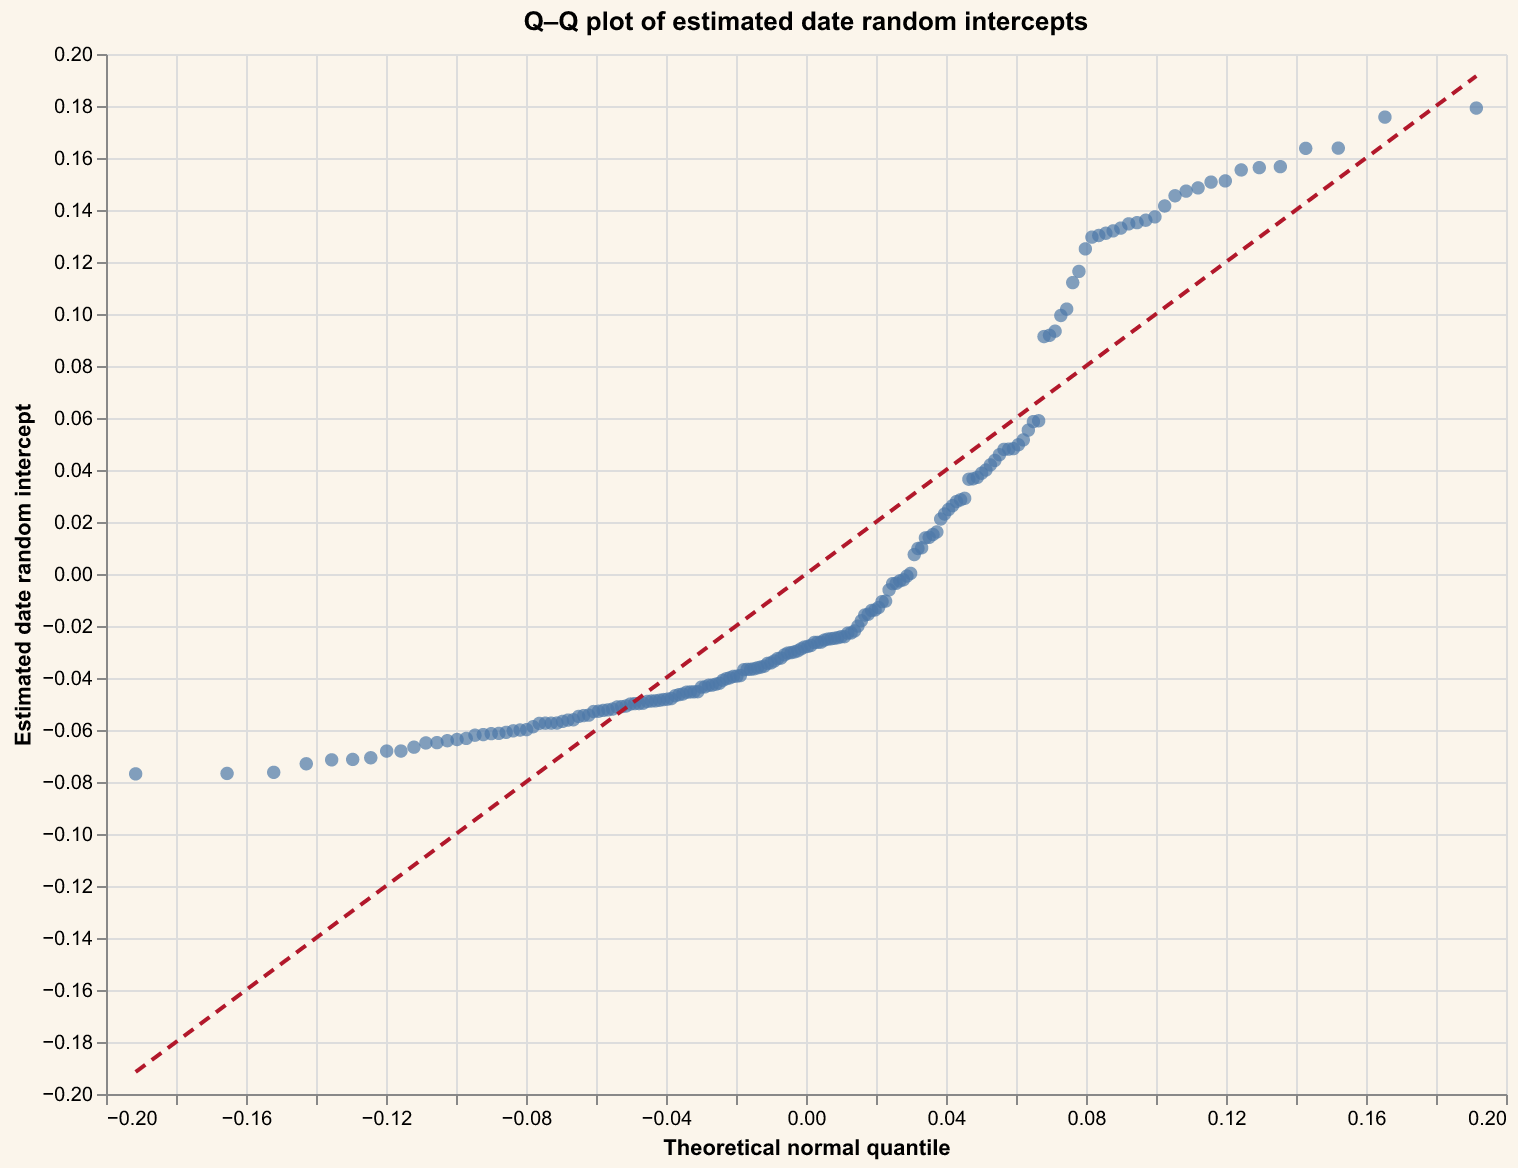
\includegraphics[keepaspectratio,alt={Date Q--Q plot}]{outputs/charts/mc3-coh-pettype-final-model/date_random_intercepts_qq.png}}

\pandocbounded{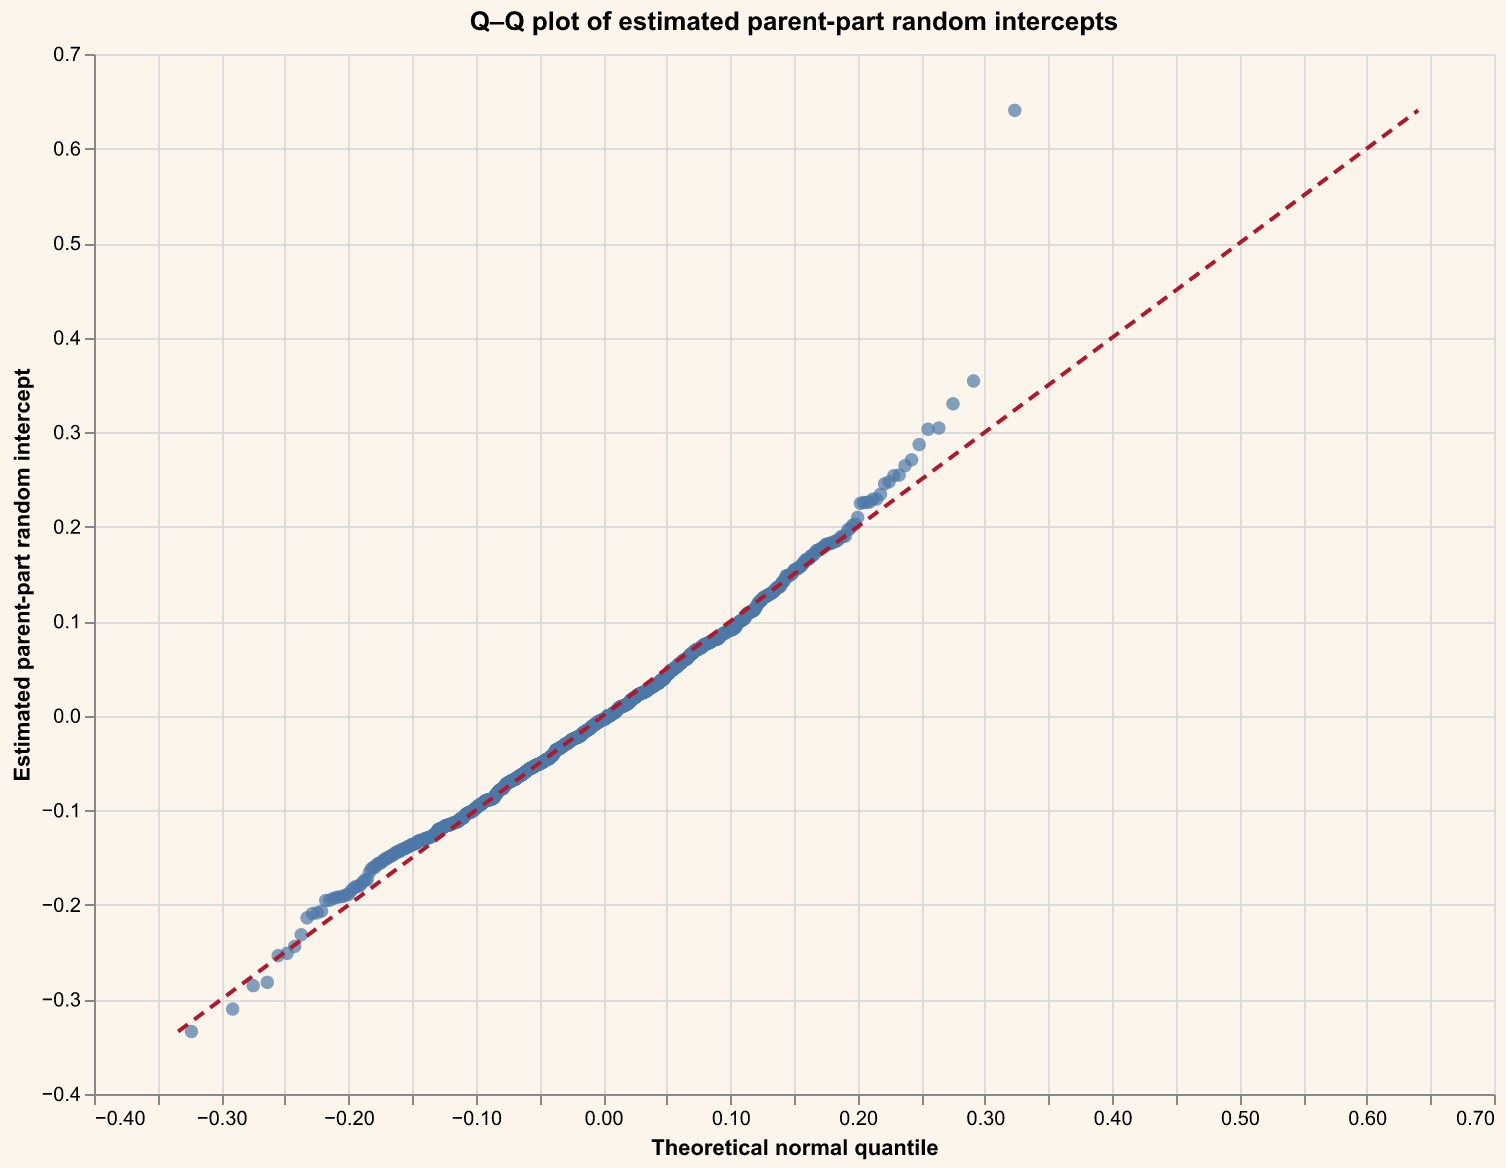
\includegraphics[keepaspectratio,alt={Parent-part Q--Q plot}]{outputs/charts/mc3-coh-pettype-final-model/parent_part_random_intercepts_qq.png}}

\pandocbounded{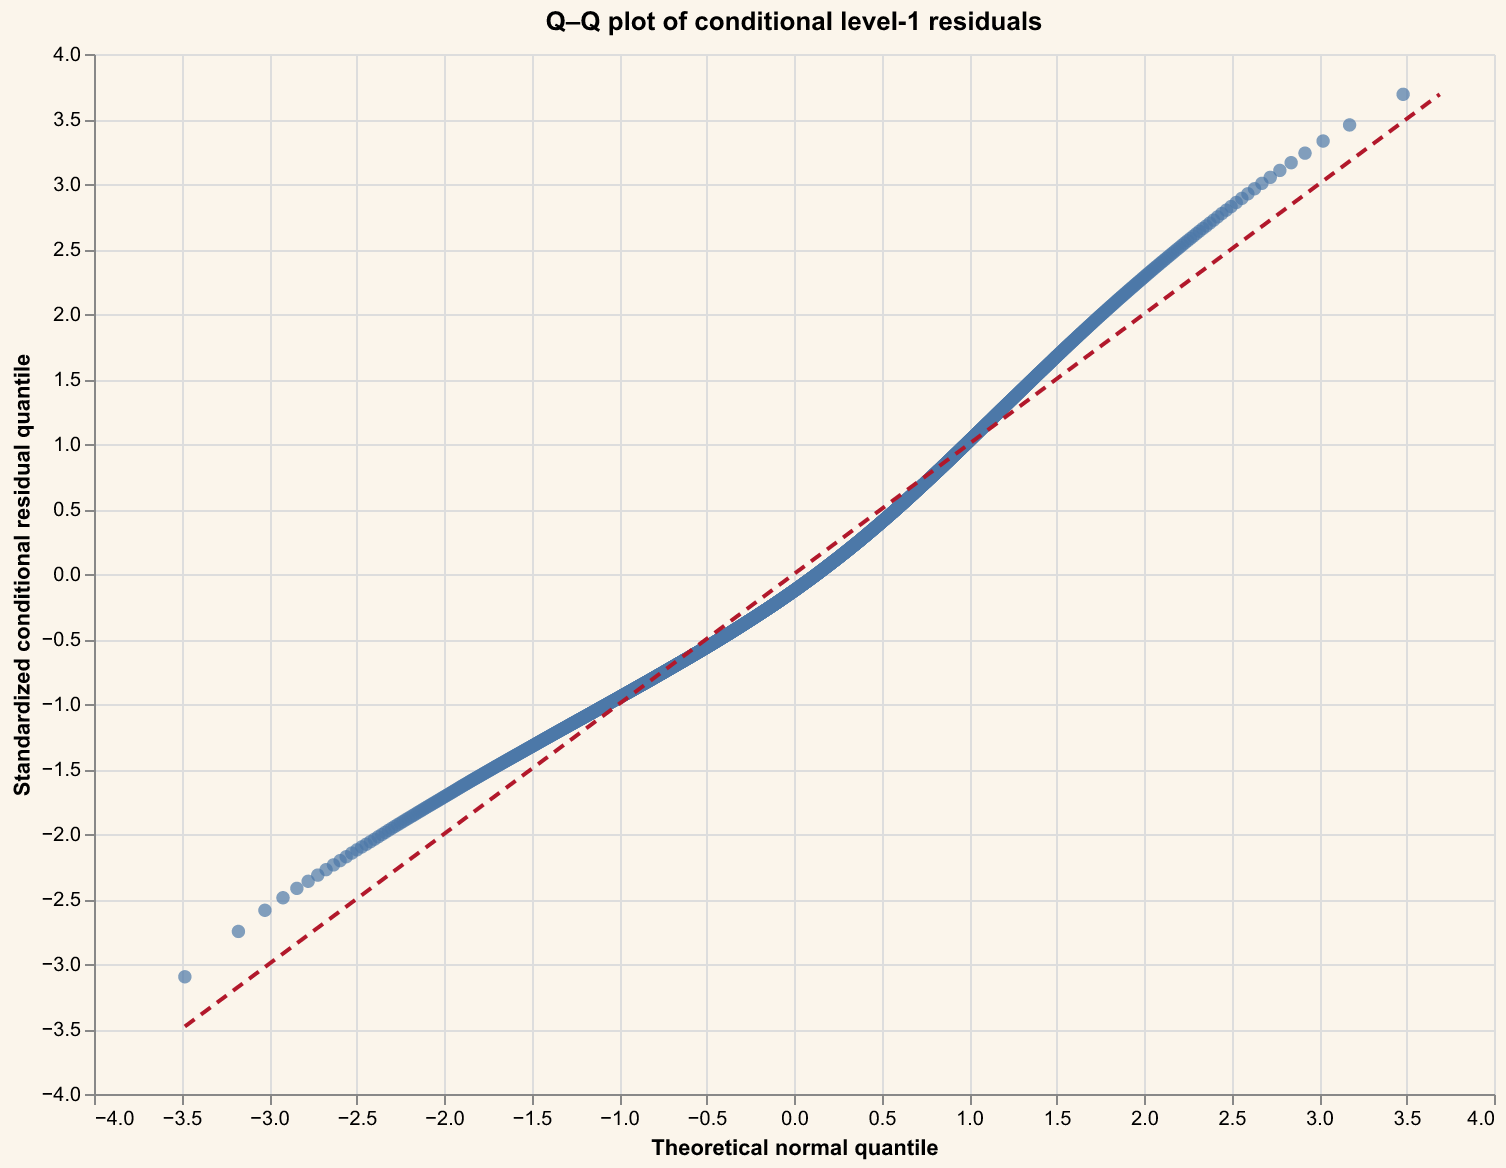
\includegraphics[keepaspectratio,alt={Residual Q--Q plot}]{outputs/charts/mc3-coh-pettype-final-model/conditional_residuals_qq.png}}

\pandocbounded{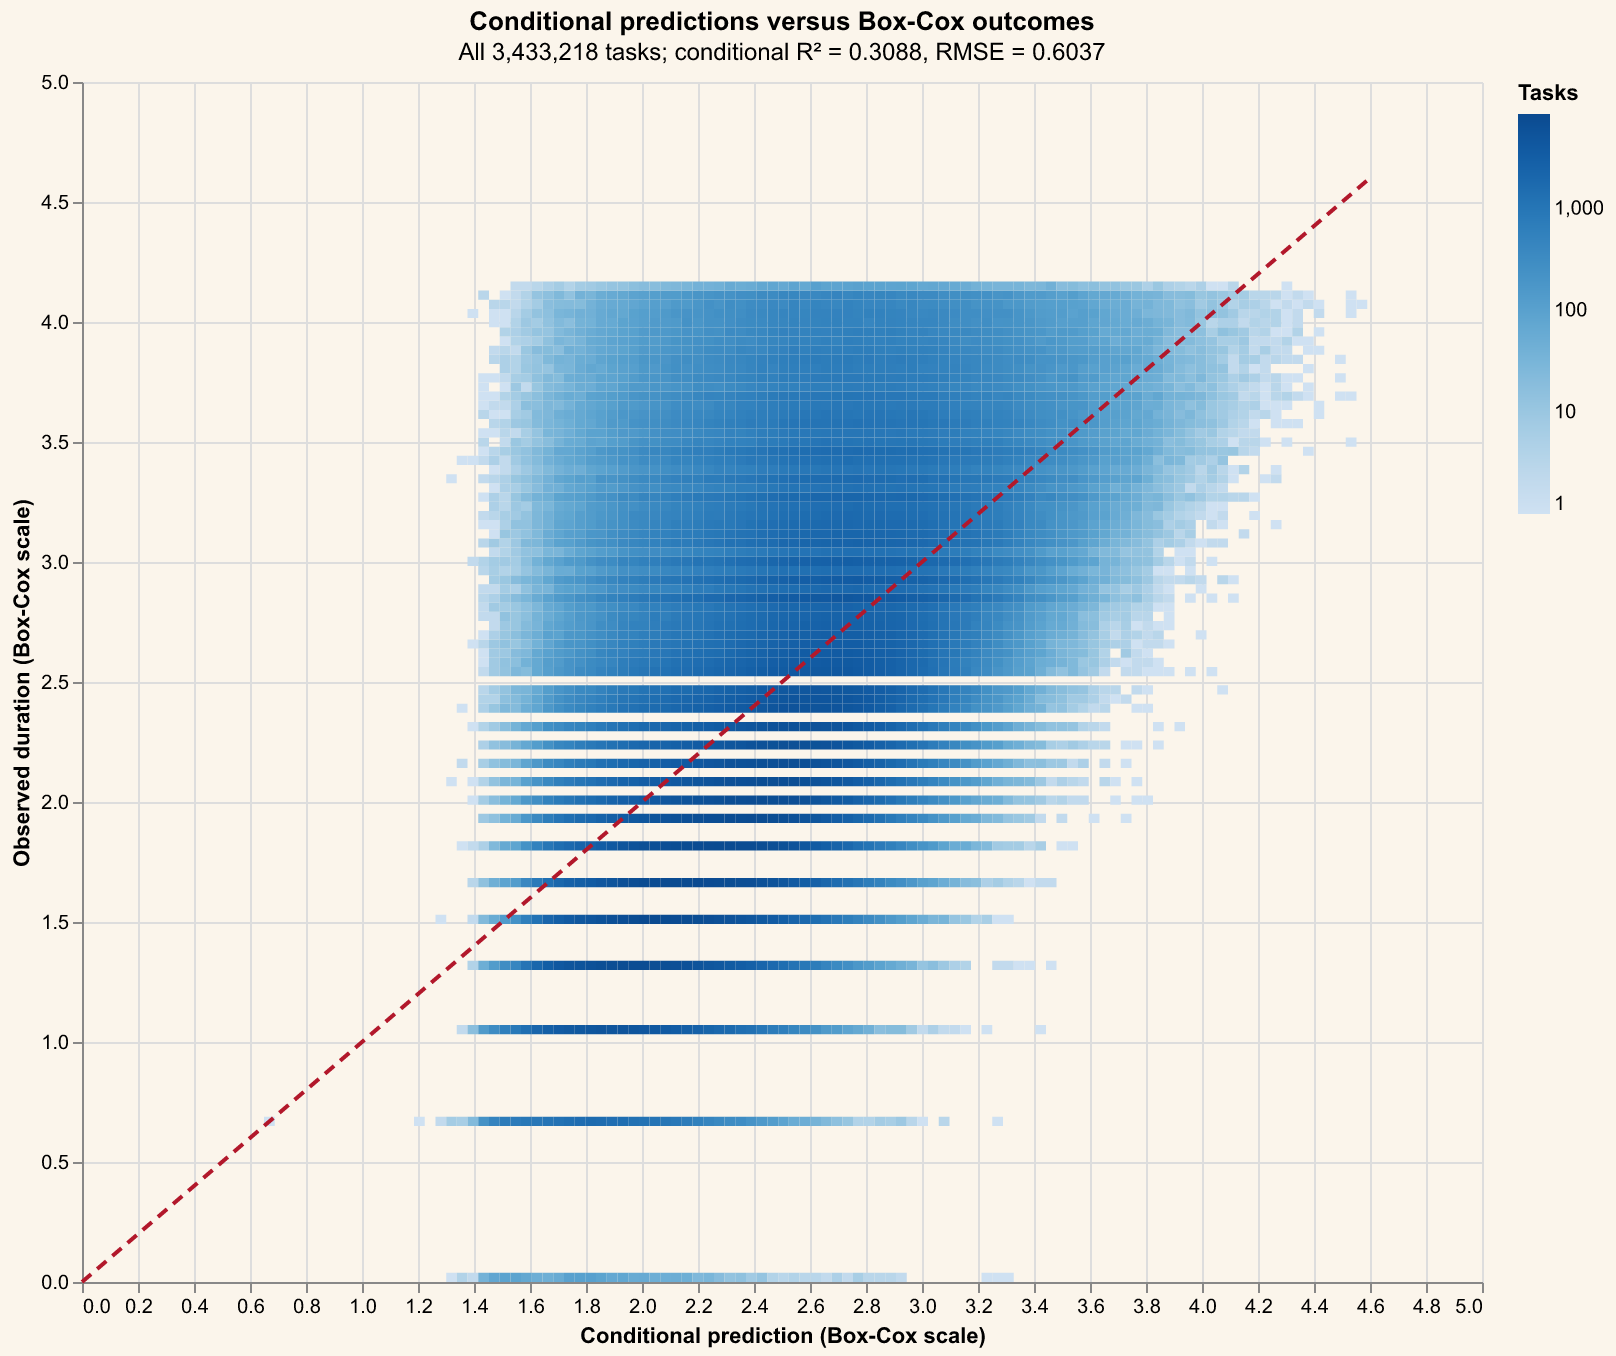
\includegraphics[keepaspectratio,alt={Predicted versus outcome}]{outputs/charts/mc3-coh-pettype-final-model/predicted_vs_boxcox_actual.png}}
